\graphicspath{{chapters/1_basicfeatures/figures/}}

\chapter{Basic features of the template}
\section{Compiling the main document}
To compile the thesis and the bibliography and obtain flawlessly working cross-references between the table of content and the main text, as well as the citations and the bibliography, run
\begin{lstlisting}
lualatex main_thesis.tex
biber main_thesis
lualatex main_thesis.tex
lualatex main_thesis.tex
\end{lstlisting}
Of course, it is not necessary to run these four commands manually. Every \LaTeX editor I ever worked with (SublimeText, VS Code, TeXstudio, TeXmaker, TeXShop and also overleaf) allows one to set \verb|lualatex| as the standard and biber as the default and for all these editors, it is also possible to define this succession of commands as the standardard build command that is executed whenever you compile your document.

\paragraph{Why lualatex?} This template is compiled with \verb|lualatex|, not \verb|pdflatex|. There a two specific reasons for that: 
(i) The \verb|fontspec| package is used to handle different font types (e.g., a sans-serif font for captions and a serif font for the main text). This package requires compilation with \verb|lualatex|. 
(ii) \verb|lualatex| has the superior storage management system, with the ability to dynamically allocate memory if needed. This is crucial when creating figures in \LaTeX with pfgplots and TikZ where simple two-dimensional surface plots can result in out-of-memory errors with \verb|pdflatex|.

It is worth noticing that there are more reasons to switch to the modern and versatile \verb|lualatex| engine besides the two examples relevant here (for example, the powerful lua language support). There are many discussions on the benefits on \href{tex.stackexchange.com}{tex.stackexchange}.

\paragraph{Why biber and biblatex?} The template uses biblatex with the biber backend. Biblatex is more modern and versatile than Bibtex.
I cannot think of a single reason why one should prefer bibtex over biblatex. The only reason bibtex is still so popular is probably because people (and, unfortunately, also some journals for which bibtex is mandatory) apparently find it hard to break their bad habits.

For a thesis with a fairly simple bibliography structure, one might achieve the desired output with bibtex, but biblatex is easier to customize. In addition, for more complex (bibliography) projects like our CRC183 proposal, with several independent bibliographies, the possibility of cross-referencing between them, chapter-specific highlighting of selected citation keys and the automatic fixing of incorrect biblatex/bibtex entries, we would have failed miserably with bibtex.
See \chapref{chap:biblatex} for details.



\section{Documentclass}
This template is build on the \href{https://ctan.org/pkg/koma-script?lang=de}{KOMA-script} class \verb|scrbook|. 
Whether one prefers the standard \verb|book| class or its KOMA-script variant \verb|scrbook| is mainly a matter of personal taste. There is general consensus that the KOMA-script bundle is an amazing package, and, personally, I find \verb|scrbook| easier to adjust to my wishes and prefer the standard layout it produces. 
The documentclass is loaded with the following options:
\begin{lstlisting}
\documentclass[numbers=noenddot, headinclude = true,
	BCOR = 12mm, DIV = 16, twoside]{scrbook}
\end{lstlisting}
Some of the options are explained below.

\subsection{Page layout without the \texttt{geometry} package}
One of the strengths of the KOMA script classes is the handling of type area and other typographic settings. The author of the classes has a background in this very area and has incorporated much of his expertise into the implementation. Here is an excerpt taken from the Koma script manual CITe: ``Various algorithms and heuristic methods for constructing an appropriate type area have been discussed in the literature. These rules are known as the `canons of page construction.' [\ldots] The result is that the
aspect ratio of the type area corresponds to the proportions of the page. [\ldots] In a two-sided document (e.g. a book), however, the entire inner margin (the margin at the spine) should be the same size as each of the two outer margins.'''

The \verb|scrbook| class automatically generates margins that are compatible with the ``canon of typographie''. The parameter that controls the width is \verb|DIV|. The larger the value, the smaller the margin. The underlying construction mechanism is explained in  
Sec.~2.2 of the KOMA script manual, and in particular Fig.~2.1.
The option \verb|headinclude = true| is considered as part of the typearea. The parameter \verb|BCOR = 12mm| adds a binding correction to the inner margin.

In particular, note that one does \emph{not} need the geometry package to adjust the page margins. In fact, when manually fixing different lengths for the margins, it is not unlikely that you violate some of the typographic rules. See also the discussion in Sec.~2.8 of Ref.~. and its closing quotation, taken from ... ``The practice of doing things oneself has long been widespread, but the results are often dubious because amateur typographers do not see what is wrong and cannot know what is important. This is how you get used to incorrect and poor typography. [...] Now the objection could be made that typography is a matter of taste. When it comes to decoration, one could perhaps accept that argument, but since typography is primarily about information, not only can mistakes irritate, but they may even cause damage.''

\paragraph{A confession} Now that I have explained in detail that it is sacrilege to violate what typographers consider to be a good type area, it is time for a confession: I am in serious violation. 
For each combination of font size, font type (e.g. sans serif or serif) and paper size there is a maximum number of characters that should be contained in a line in order not to impair readability. This yields a maximum DIV value. I am using a value (16) that is way too large (when compiling, one gets a \verb|Bad type area settings!|-warning, together with the proposal to decrease the \verb|DIV| value. I personally prefer the smaller-margin version and justify my decision with the fact that the maximum number of characters per line are rather values for inexperienced readers.


\section{Structure of the thesis}

According to the \href{https://mathnat.uni-koeln.de/sites/dekanat/official/Ordnungen/Promotionsordnung_2020.pdf}{`Promotionsordnung der math.-nat. Fakultät (2020)'} (PO2020), a thesis must include
\begin{itemize}
	\item a cover / title page,
	\item an abstract (according to the PO2020, one does not need a german and an english abstract, the latter is sufficient),
	\item several chapters including an introduction, presentation of results and a discussion,
	\item the statement from §7 Absatz 8, PO2020, together with a list of publications.
\end{itemize}

The published version (i.e., not your inital submission, but the one you publish after your defense) must contain a statement that the thesis was accepted by the faculty. This should be printed either on the title page or its back (see this template for an example).

It is common to also include a thesis outline and acknowledgements. There is no universal consensus on where the best place for the acknowledgments is, I put it between the bibliography and the closing statement, but have also seen otherwise (for example directly after the title page, before the abstract, I think if I had to write my thesis again, I would pick that option).

Usually, acknowledgments and abstract do not go into the table of contents. Regarding the closing statement, there is apparently no clear consesus, I decided to not include it in the table of content. However, I wanted all three parts to have an individual entry in the table of content of the pdf-file, i.e., the content that is displayed in the content pane / left column of a pdf-reader, see Fig. XX.

The following commands are used ...
\verb|\addcontentsline{toc}{chapter}{Bibliography}|
\verb|\pdfbookmark{Abstract}{abstract}|


Sometimes one needs a \verb|\phantomsection| to ensure that one jumbs to the correct section when clicking on the corresponding entry in the pdf-table of content.

It can happen that -- e.g. after you inserted a part page -- something is odd with the hierarchy...

\begin{lstlisting}
\makeatletter
\def\toclevel@chapter{-1}
\makeatother
\end{lstlisting}
or 
\begin{lstlisting}
\usepackage{bookmark}
...

\bookmarksetup{startatroot}
\chapter{conclusion}
\end{lstlisting}


\begin{figure}
	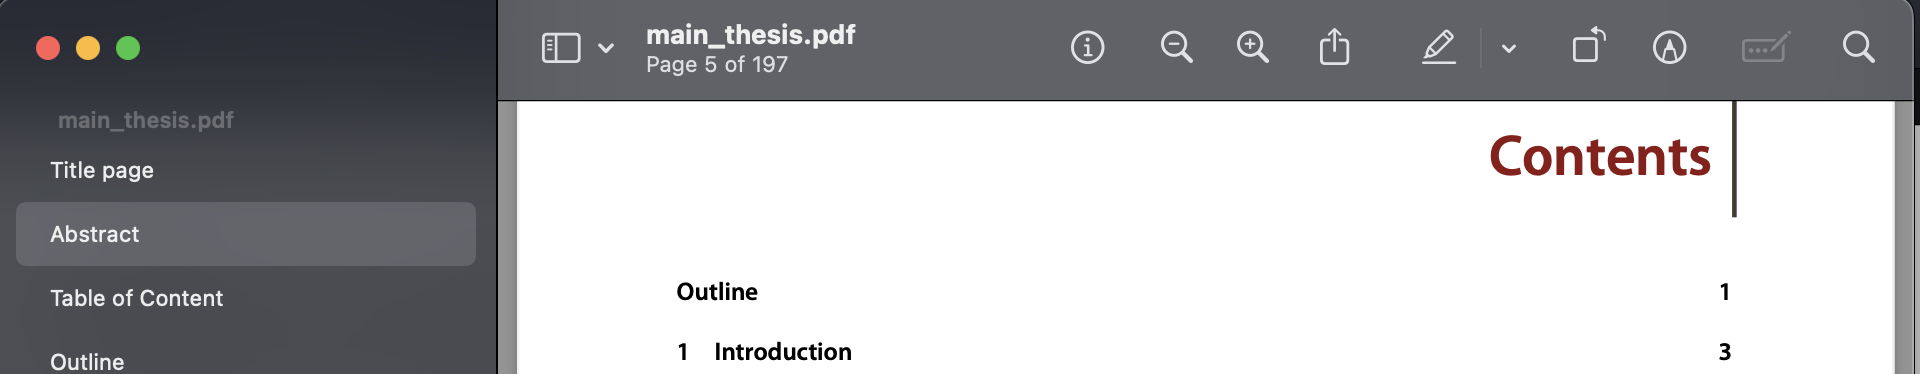
\includegraphics[width = \textwidth]{pdf-toc.png}
\end{figure}

\begin{table}
	\centering 
	\caption{\textbf{Structure of the thesis.}}
	\label{tab:table2}
	\vspace{5ex}
	\begin{tabular}{lccccc} 
		\toprule
		 & page numbers & even/odd & in ToC & in pdf ToC & numbered  \\ 
		\midrule 
		Titlepage I  & none & odd & \color{bqred}\XSolidBrush& \color{bqgreen} \CheckmarkBold &\color{bqred} \XSolidBrush\\
		Titlepage II & none & even & \color{bqred}\XSolidBrush& \color{bqred}\XSolidBrush& \color{bqred}\XSolidBrush\\
		Abstract & none & odd & \color{bqred}\XSolidBrush& \color{bqgreen}\CheckmarkBold & \color{bqred}\XSolidBrush\\
		Table of Contents & roman & odd & \color{bqred}\XSolidBrush& \color{bqgreen}\CheckmarkBold &\color{bqred} \XSolidBrush\\
		Outline & arabic & odd &\color{bqgreen} \CheckmarkBold &\color{bqgreen} \CheckmarkBold & \color{bqred}\XSolidBrush\\
		Part page & none & odd & \color{bqgreen}\CheckmarkBold & \color{bqgreen}\CheckmarkBold & roman letters\\
		Chaptes & arabic & odd & \color{bqgreen}\CheckmarkBold &\color{bqgreen} \CheckmarkBold & numbers\\
		Appendices & arabic & odd & \color{bqgreen}\CheckmarkBold &\color{bqgreen} \CheckmarkBold & letters\\
		Bibliography & arabic & odd & \color{bqgreen}\CheckmarkBold & \color{bqgreen}\CheckmarkBold & \color{bqred}\XSolidBrush\\
		Acknowledgements & none & odd & \color{bqred}\XSolidBrush& \color{bqgreen}\CheckmarkBold & \color{bqred}\XSolidBrush\\
		Erklärung & none & odd & \color{bqred}\XSolidBrush&\color{bqgreen} \CheckmarkBold & \color{bqred}\XSolidBrush\\
		\bottomrule
	\end{tabular}
\end{table}

\section{Folder structure of the template}


\section{``Outer theme'' layouting}

\subsection{Chapter headings}

\subsection{Part pages}

\subsection{Header}


\chapter{``Inner theme'' layouting, formatting and style}
\section{Math environments}
\subsection{The golden rules}
\subsection{Other}
indices, mathrm, eqnarray vs. align, spacing after ..., displaying huge numbers.
\section{Tables}
\subsection{Booktabs}
\subsection{Colored rows / cells}
\section{Figures}
\subsection{Side by side}
\subsection{Hyperlinks to subpanels}
\section{Fine-tuning}
Immer wenn ich einen der folgenden Fehler sehe, dann baut sich bei mir direkt der Gedanke auf, dass der Autor jetzt direkt in der Bringschuld ist, mir zu beweisen, dass er kein Idiot ist. Mit anderen Worten: Wenn ich so etwas sehe kriege ich schlechte Laune und bin dem Inhalte gegenüber nicht mehr neutral (sogar mehr noch, als wenn ich inhaltliche Fehler sehe). Klingt übertrieben? Mag sein, aber wenn man seine Leserschaft nicht kennt, sollte man sich trotzdem Mühe geben, es direkt richtig zu machen. Wer weiß an wen man gerät.
\subsection{Quotation marks}
\subsection{Hyphens}
\subsection{nonlinear vs. non-linear}
\subsection{Orphans and widows}

\chapter{Colors}
\chapter{Bibliography with biblatex}\label{chap:biblatex}

\chapter{General advice}
use newcommands for ...
read the promotionsordnung
whatever you do, do it consistently
In case of trouble, first step is to delete cached files


In this first chapter, I briefly describe some general properties of the template: How to compile, what is the general structure, general remark about the page layouts, etc.

\section{Compilation, documentclass and page layout}

To compile the entire document, including the bibliography, run
\begin{lstlisting}
lualatex main_thesis.tex
biber main_thesis
lualatex main_thesis.tex
lualatex main_thesis.tex
\end{lstlisting}

This should result in a pdf-document where all references are correctly displayed and all cross-links between the bibliography in the main text works flawlessly.
Of course, it should not be necessary to run these four commands manually in the terminal. Every tex editor I ever used (SublimeText, VS Code, TeXstudio, TeXmaker, TeXlive) allows one to choose 
this succession of four commands as the standard build command that is executed whenever you compile your document.


\subsection{The document class}
This template uses the KOMA-script class \verb|scrbook|. There are many discussion on the pros and cons of KOMA-script classes over the regular \verb|book| class. I personally find the \verb|scrbook| easier to adjust to my wishes and slighly prefer the standard layout it produces. There is general consensus that the KOMA-script is a great bundle.

\paragraph{Page layout} One often sees people using the \verb|geometry| package to adjust the margins of the page. That is certainly a cool package, but in my opinion, don't use it, unless you really now what you are doing. There are surprisingly many things you can screw up, or stated otherwise, typographers have thought about good guidelines for layouting a page for years, so don't screw it up fahrlaessig.  
Here is a quotation from the KOMA-script manual:
``'Various algorithms and heuristic methods for constructing an appropriate type area have been
discussed in the literature. These rules are known as the ``canons of page construction.'' \ldots The result is that the
aspect ratio of the type area corresponds to the proportions of the page. In a one-sided document,
the left and right margins should have equal widths, while the ratio of the top and bottom margins
should be 1:2. In a two-sided document (e.g. a book), however, the entire inner margin (the margin at the spine) should be the same size as each of the two outer margins \ldots.'

The easiest way to make sure that the text area has the same ratio as the page is as follows:

\href{https://markov.htwsaar.de/tex-archive/macros/latex/contrib/koma-script/doc/scrguide-en.pdf}{How page layout is calculated.}

\begin{lstlisting}
\documentclass[BCOR = 12mm, DIV = 16, ...]{scrbook}
\end{lstlisting}


but that gives the Warning

I personnaly find that the margins produced with the default settings are too wide, therefore I use the large DIV value of 16 (I am sure that the KOMA-script author would consider this as a sacrileg). This gives me the following warning when I compile.

\begin{lstlisting}
Package typearea Warning: Bad type area settings! The detected line width is about 17\% larger than the heuristically estimated maximum limit of typographical good line width. You should e.g. decrease DIV, increase fontsize or change papersize.
\end{lstlisting}

But as I am quite happy with the final result, I just ignore these messages.



\blindtext
\section{Here is a section}
\blindtext
\subsection{Here is a subsection}
\blindtext
\subsubsection{This is a subsubsection}
I never use subsubsections.
\paragraph{Paragraph} but sometimes I use paragraphs.
\section{How to cite papers.}
Blablabla, have a look at this cool paper \cite{berke_transmon_2022}. Note the `P' because it is one of \highlight{my} papers. Here is a regular paper \cite{aruteQuantumSupremacyUsing2019a} with a million authors, such that BibLaTeX uses (depending on your settings) \textit{et al.} and here is another paper \cite{magesan_effective_2020} with only two authors. Finally, here is one of my papers that is not yet published, and, therefore, I decided that it deserves its own category \cite{inpreparation}.

\section{How to make nice tables?}
Most importantly, do not use vertical rules!
From `The Chicago Manual of Style' \cite{chicagoMOS}: ``To produce a clear, professional-looking table, rules should be used sparingly. Many tables will require just three rules, all of them horizontal—one at the very top of the table, below the title and above the column heads; one just below the column heads; and one at the bottom of the table, along the bottom of the last row, above any notes to the table. (\ldots) Vertical rules should be used sparingly (\ldots).'' 
Use the \verb|booktabs| package, see  \href{https://ctan.org/pkg/booktabs}{here} for the documentation and \href{https://nhigham.com/2019/11/19/better-latex-tables-with-booktabs/}{here} or \href{}{} for some examples and a discussion why \verb|booktabs| is the way to go. Remember that table captions usually go above the table. See \tabref{tab:table1} for an example with multiple hierachy levels in $x$ and $y$ direction and \tabref{tab:table2} for an example of a side-by-side table with colored rows.

\begin{table}
	
	\centering
	\caption{\textbf{Example for table with different hierachy levels in $x$ and $y$ direction.} \blindtext}
	\label{tab:table1}
	\vspace{5ex}
	\begin{tabular}{@{}rrrrcrrr@{}}\toprule
		& \multicolumn{3}{c}{$w = 8$} & \phantom{abc}& \multicolumn{3}{c}{$w = 16$} \\
		\cmidrule{2-4} \cmidrule{6-8}
		& $t=0$ & $t=1$ & $t=2$ && $t=0$ & $t=1$ & $t=2$\\ 
		\midrule
		$\mathrm{dir}=1$\\
		$c$ & 0.0790 & 0.1692 & 0.2945 && 0.3670 & 0.7187 & 3.1815 \\
		$c$ & -0.8651& 50.0476& 5.9384&& -9.0714& 297.0923& 46.2143\\
		$c$ & 124.2756& -50.9612& -14.2721&& 128.2265& -630.5455& -381.0930\\
		$\mathrm{dir}=0$\\
		$c$ & 0.0357& 1.2473& 0.2119&& 0.3593& -0.2755& 2.1764\\
		$c$ & -17.9048& -37.1111& 8.8591&& -30.7381& -9.5952& -3.0000\\
		$c$ & 105.5518& 232.1160& -94.7351&& 100.2497& 141.2778& -259.7326\\
		\bottomrule
	\end{tabular}

\end{table}

\begin{table}
	\centering 
	\caption{\textbf{Example of side-by-side table and colored rows.} \blindtext}
	\label{tab:table2}
	\vspace{5ex}
	\begin{tabular}{ccccrr} 
		\toprule
		$l_1$ & $l_2$ & $l_3$ & $l_4$ & $\Delta N_\text{ex}$ & $|\langle \psi | \op{H}_\text{int} | \phi \rangle|$  \\ 
		\midrule 
		\rowcolor{pqred} 0 & 1 & 3 & 0 & 0 & ---\\
		0 & 0 & 0 & 0 & $-4$ & 0.04\\
		0 & 0 & 2 & 0 & $-2$ & 1.88\\
		\rowcolor{pqblue} 0 & 0 & 4 & 0 & 0 & 2.06\\
		0 & 0 & 6 & 0 & 2 & 0.32\\
		0 & 0 & 8 & 0 & 4 & 0.09\\
		0 & 1 & 0 & 1 & $-2$ & 0.04\\
		\rowcolor{pqyellow} 0 & 1 & 0 & 3 & 0 & 0.002\\
		0 & 1 & 0 & 5 & 2 & 0.0001\\
		0 & 1 & 0 & 7 & 4 & 0.00002\\
		\rowcolor{pqblue} 0 & 1 & 2 & 1 & 0 & 1.89\\
		\bottomrule
	\end{tabular}
	\hspace{0.5cm}
	\begin{tabular}{ccccrr} 
		\toprule
		$l_1$ & $l_2$ & $l_3$ & $l_4$ & $\Delta N_\text{ex}$ & $|\langle \psi | \op{H}_\text{int} | \phi \rangle|$  \\ 
		\midrule 
		0 & 2 & 0 & 0 & $-2$ & 0.06\\
		\rowcolor{pqblue} 0 & 2 & 2 & 0 & 0 & 2.57\\
		0 & 2 & 4 & 0 & 2 & 2.82\\
		0 & 2 & 6 & 0 & 4 & 0.44\\
		\rowcolor{pqyellow} 0 & 4 & 0 & 0 & 0 & 0.003\\
		0 & 4 & 2 & 0 & 2 & 0.15\\
		0 & 4 & 4 & 0 & 4 & 0.17\\
		0 & 6 & 0 & 0 & 2 & 0.0005\\
		0 & 6 & 2 & 0 & 4 & 0.02\\
		0 & 8 & 0 & 0 & 4 & 0.0001\\
		\rowcolor{pqblue} 1 & 0 & 3 & 0 & 0 & 1.17\\
		\bottomrule
	\end{tabular}
\end{table}


\chapter{Notes on the use of colors}

Selecting well-suited colors is a surprisingly complex challenge. Besides the requirement to be aesthetically pleasing, the color schemes should at best
\begin{itemize}
	\item be distinct for color-blind readers,
	\item work in monochrome print out,
	\item work on screen and paper,
	\item respect `semantic resonances' \cite{linSelectingSemanticallyResonantColors2013} (e.g., `blue=cold',`red=hot' \footnote{Note that such associations can vary depending on cultural conditioning. The association of `blue' with `cold' is nearly universal, but, e.g., the colour of mourning is white in Japan, but black in many western cultures.}),
	\item be printer-friendly (`RGB vs. CMYK' issue).
\end{itemize}
The first point is probably the most important, considering that, for example, 6\% of all males have deutan color vision deficiency (`green-blindness'). Fortunately, there are many very good color picking tools, or predesigned color schemes tailored to colorblind people.
The references and tools that I have used most often are \href{https://personal.sron.nl/~pault/#sec:greyscale_conversion}{`Paul Tol's Notes'} and \href{https://colorbrewer2.org/#type=sequential&scheme=BuGn&n=3}{ColorBrewer}. 
The color palettes presented there have made it to a certain reputation. In `Paul Tol's notes', you will also find some details worth reading about the different types of color blindness and greyscale conversion.
Finally, \href{https://www.vis4.net/palettes/}{vis4.net} is a advanced and powerful tool based on \href{https://github.com/gka/chroma.js}{chroma.js} that helps you designing your own color palette, and it even shows you the perception of the chosen colors with the most frequent forms of color blindness. However, I was usually completely satisfied with the first two references.

In my thesis, I had four different main use cases for colors, some with specific sub-cases:
\begin{itemize}
	\item Line plots:
		\begin{itemize}
			\item qualitative,
			\item pairwise,
			\item sequential. 
		\end{itemize}
	\item surface plots:
		\begin{itemize}
			\item qualitative,
			\item divergent,
			\item sequential. 
		\end{itemize}
	\item colored text or text on colored background, e.g. filled cells in tables,
	\item other design elements or drawings.
\end{itemize}
For the last point (e.g. heading colors, link colors, or sketch of, e.g., a physical system like a pendulum, i.e., cases where there is no loss of information to fear if colors are perceived incorrectly) I have taken as the only criterion my personal taste. The other points are explained in more detail below.


\section{Define your own commands}
\verb|\figref|

\section{Example of figures and side-by-side figures.}

\section{Some stylistic advices}
Below is a collection of stilistic questions I have thought about for too long.
\subsection{Hyphen vs. en dash vs. em dash}
There a three lengths of hyphens, the regular hyphen \verb|-|, the en dash \verb|--| and the em dash \verb|---|.
This is what they look like: - vs. -- vs. ---.
In accordance with the Chicago manual of style, I used the hyphen only to connect words that function together as a single concept or work together as a joint modifier, i.e., `well-defined concept' or `collision-free device'. Never use the single hyphen similar to brackets.
The main application for the en dash is to connect things that are related by some form of distance, e.g. `pages 12--17', the `May--September issue of journal \ldots', the cycling race Milan--San Remo `or `a coupling strength of 10--15 MHz' (although in the last example I would rather write `10 to 15 MHz'. 
A use case I never encountered: an en dash is used in place of a hyphen in a compound adjective. Specifically, an en dash is preferred when one element of the compound is itself an open compound. For example, the prefix post- is usually connected to the following word with a hyphen, but to connect it to the compound noun World War II, it’s better to use an en dash, i.e., post--World War II vs. post-World War II.

The em dash should be used to separate additional thoughts---like this. Here is an example from my thesis: `Here, we argue that the insights gained for the simpler model---in particular, the existence of a quantum chaotic region for too low disorder---retain their validity for more elaborate frequency arrangements and geometries.' I use the em dashs without spaces as is usually recommended however some style guides --- not sure which one --- recommend the use of spaces (some times -- as here -- one encounters the combination of en dashes with spaces.

As always, the most important thing is consistency. Once you have decided on a variant, you should use it consistently everywhere and always.

\subsection{Nonlinear vs. non-linear and related issues}
The prefix `non' appears very often and with many different following words. My impression was that it is not treated uniformly in the literature (even by the same authors) and that one finds both variants. In fact, in American English (AE), the hyphen is mostly omitted, whereas in British English (BE) it is commonly used. Compare e.g., the two reviews \cite{abaninRecentProgressManybody2017} and \cite{abaninColloquiumManybodyLocalization2019}. Ref.~\cite{abaninRecentProgressManybody2017} was published by Annals of Physics (Berlin) which belongs to the german Wiley-VCH publisher and uses BE. Therefore one finds \emph{non-quilibrium,non-entangled,non-uniform,non-thermal,non-ergodic,non-local,non-trivial,non-interacting,non-Abelian,} etc.
Ref.~\cite{abaninColloquiumManybodyLocalization2019} was published in Reviews of modern physics, an APS journal. In consequence, they write \emph{nonequilibrium,nonzero,noninteracting,nonuniform,nonthermal,nonvanishing,nonlocal,nonthermalizing}, but however, they write \emph{non-Abelian}. I went for the AE option, because I used AE everywhere else (behavior, neighbor, gray, etc.).
When browsing papers to find out how issues like this are handled, the best idea is not to take the arXiv versions, as there is often no consistency even within a single paper, but the published versions that have undergone some form of post-editing by the publisher.


\subsection{Indices}
$E_\text{kin}$ vs $E_\mathrm{kin}$ vs $E_{kin}$. Or even worse: $cos (x) $ vs. $\cos (x)$, and $exp (x) $ vs. $\exp (x)$
$E_A$ that is fine. But as soon as you have more than one letter $E_\text{potential}$ vs. $E_{potential}$


\subsection{Math as prose}
I would like to remind you of the wise rules, provided by David Mermin himself, as a shining light in the darkness of mathematical typesetting. Let me quote directly from his epoch-making work:
\paragraph{Rule 1 (Fisher's rule)} (\dots) Number all displayed equations. The most common violation of Fisher's rule is the misguided practice of numbering only those displayed equations to which the text subsequently refers back. (\dots)
\paragraph{Rule 2 (Good Samaritan rule)}(\dots) When referring to an equation identify it by a phrase as well as a number. No compassionate and helpful person would herald the arrival of Eq.~(7.38) by saying ``inserting (2.47) and (3.51) into (5.13)'' when it is possible to say ``inserting the form (2.47) of the electricfield \textbf{E} and the Lindhard form (3.51)\dots''. (\dots) Consistent use of the Good Samaritan rule might well increase the lenght of your paper by a few percent. But admit it. Your paper is already to long by at least 30\% because you were in such a rush to get it out (\ldots).
\paragraph{Rule 3 (Math is prose rule)} (\dots) End a displayed equation with a punctuation mark. It is implicit in this statement that the absence of a punctuation mark is itself a degenerate form of punctuation that, like periods, commas or semicolons, can be used \emph{provided it makes sense.}

\section{Structure of the thesis}

If you are reading this, you are probably writing your thesis according to the rules set in the \href{https://mathnat.uni-koeln.de/sites/dekanat/official/Ordnungen/Promotionsordnung_2020.pdf}{Promotionsordnung 2020}. 
According to the Promotionsordnung, there are a few mandatory sections that must be included in your thesis:

Die Veröffentlichung muss auf dem Titelblatt oder auf der Rückseite des Titelblatts einen
Hinweis enthalten, aus der oder dem hervorgeht, dass es sich um eine von der Mathematisch-
Naturwissenschaftlichen Fakultät der Universität zu Köln angenommene Dissertation handelt;
dabei ist das Jahr der Disputation zu nennen.


